\chapter{Applications in Cryptanalysis}
\label{chp:application_in_cryptanalysis} 

\section{The vulnerability in GnuPG v1.4.15}\label{sec:vulnerability_gnupg}

\subsection{Subsection}\label{sec:first_ssection}


\section{The attack}\label{sec:attack}


\section{Chosen plaintext}\label{sec:chosen_plaintext}

\begin{wrapfigure}{r}{1\textwidth}
    \centering
    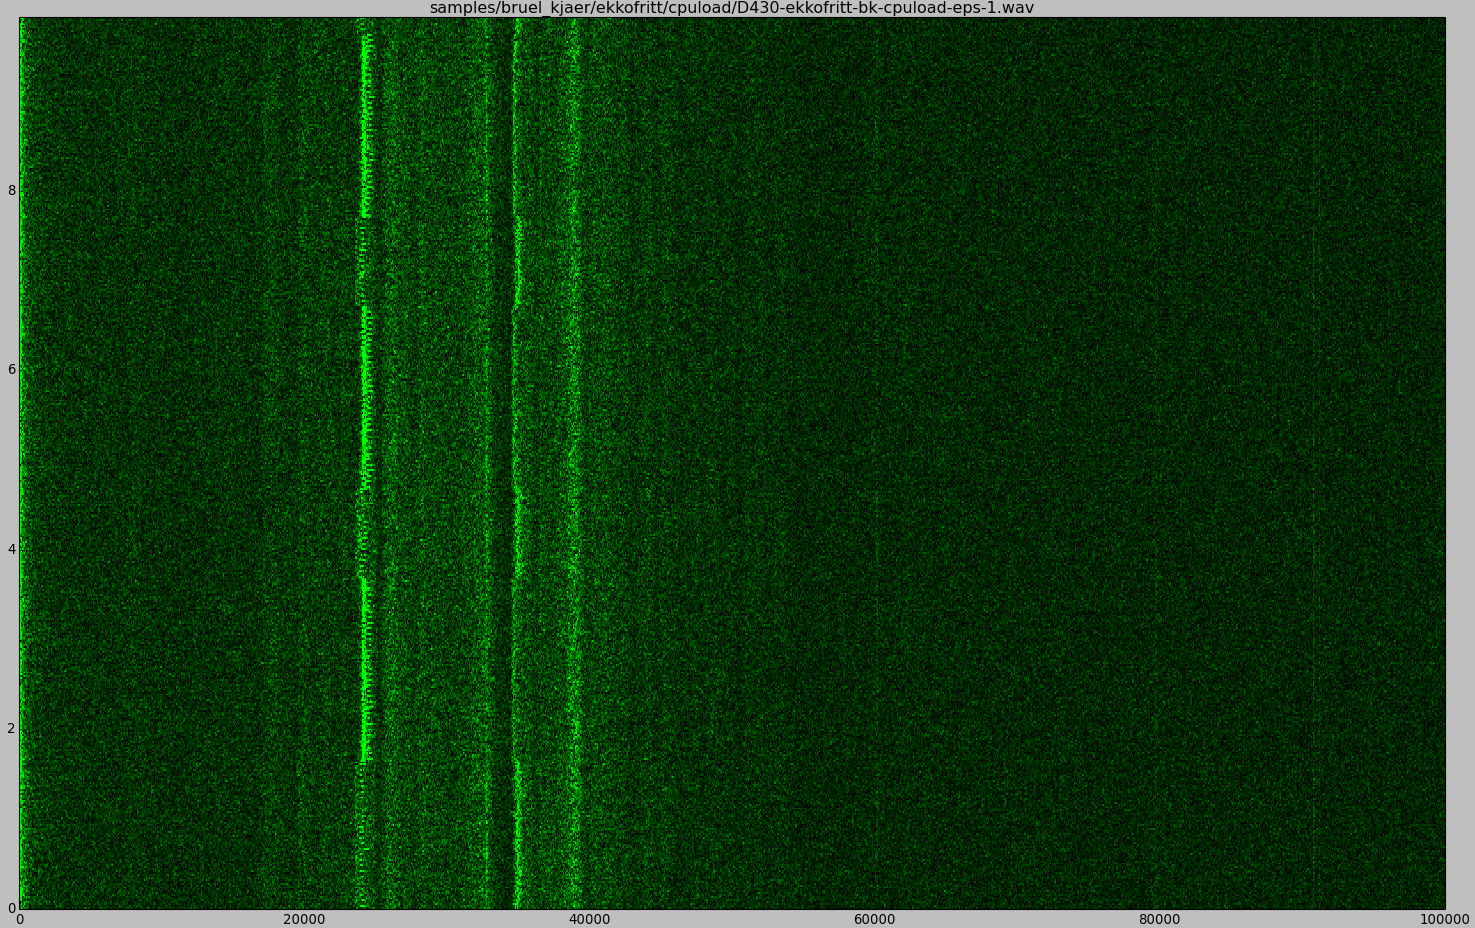
\includegraphics[width=1\linewidth]{D430-ekkofritt-bk-cpuload-eps-1.png}
    \caption{Acoustic recording (10 sec, 0-100kHz) of the Dell D430 when running a full CPU load. The recording was made in an anechoic chamber using the Brüel\&Kjær 4939 microphone with the NI myDAQ. }
    \label{fig:D430-ekkofritt-bk-cpuload-eps-1}
\end{wrapfigure}

\begin{wrapfigure}{r}{1\textwidth}
    \centering
    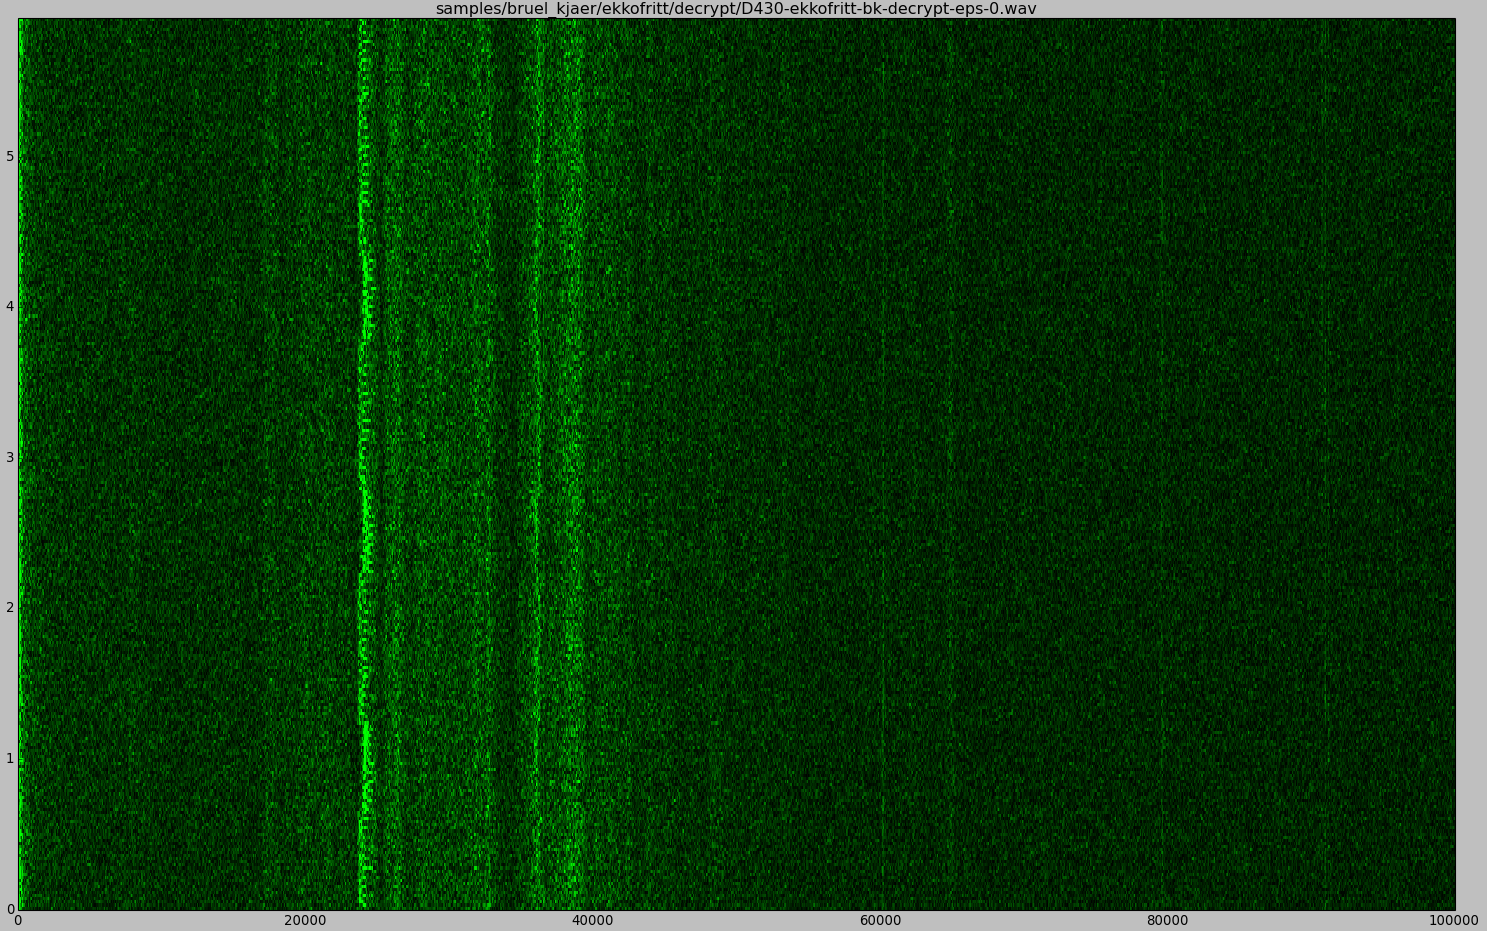
\includegraphics[width=1\linewidth]{D430-ekkofritt-bk-decrypt-eps-0.png}
    \caption{Acoustic recording (6 sec, 0-100kHz) of the Dell D430 when running a dycrypt. The recording was made in an anechoic chamber using the Brüel\&Kjær 4939 microphone with the NI myDAQ. }
    \label{fig:D430-ekkofritt-bk-decrypt-eps-0}
\end{wrapfigure}

\begin{wrapfigure}{r}{1\textwidth}
    \centering
    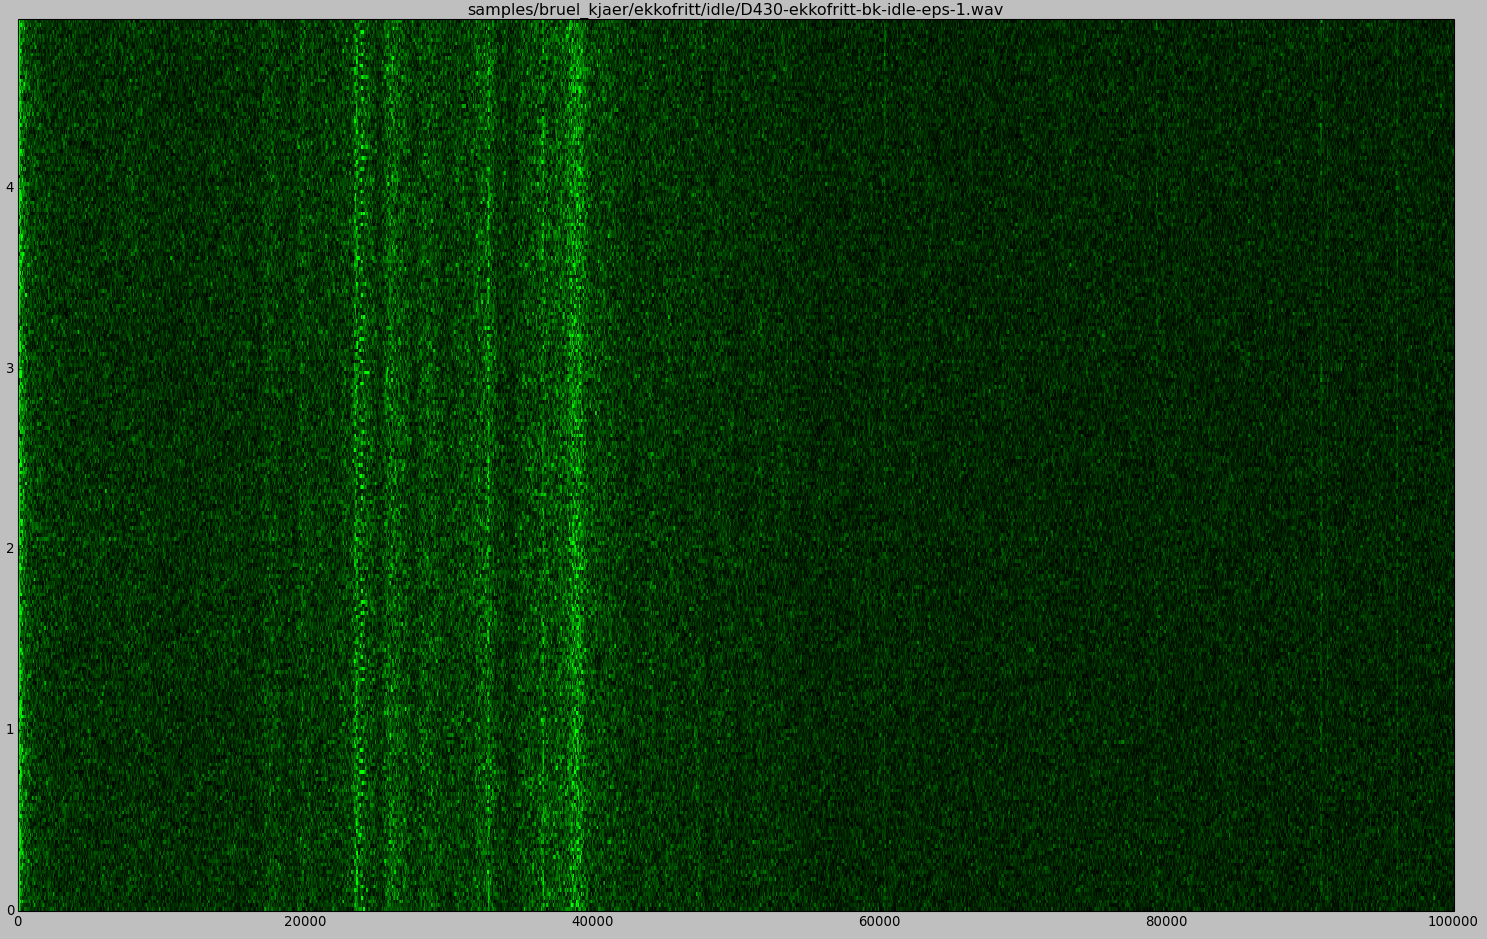
\includegraphics[width=1\linewidth]{D430-ekkofritt-bk-idle-eps-1.png}
    \caption{Acoustic recording (5 sec, 0-100kHz) of the Dell D430 when idle. The recording was made in an anechoic chamber using the Brüel\&Kjær 4939 microphone with the NI myDAQ. }
    \label{fig:D430-ekkofritt-bk-idle-eps-1}
\end{wrapfigure}


\begin{wrapfigure}{r}{1\textwidth}
	\begin{subfigure}{0.5\textwidth}
	    \centering
	    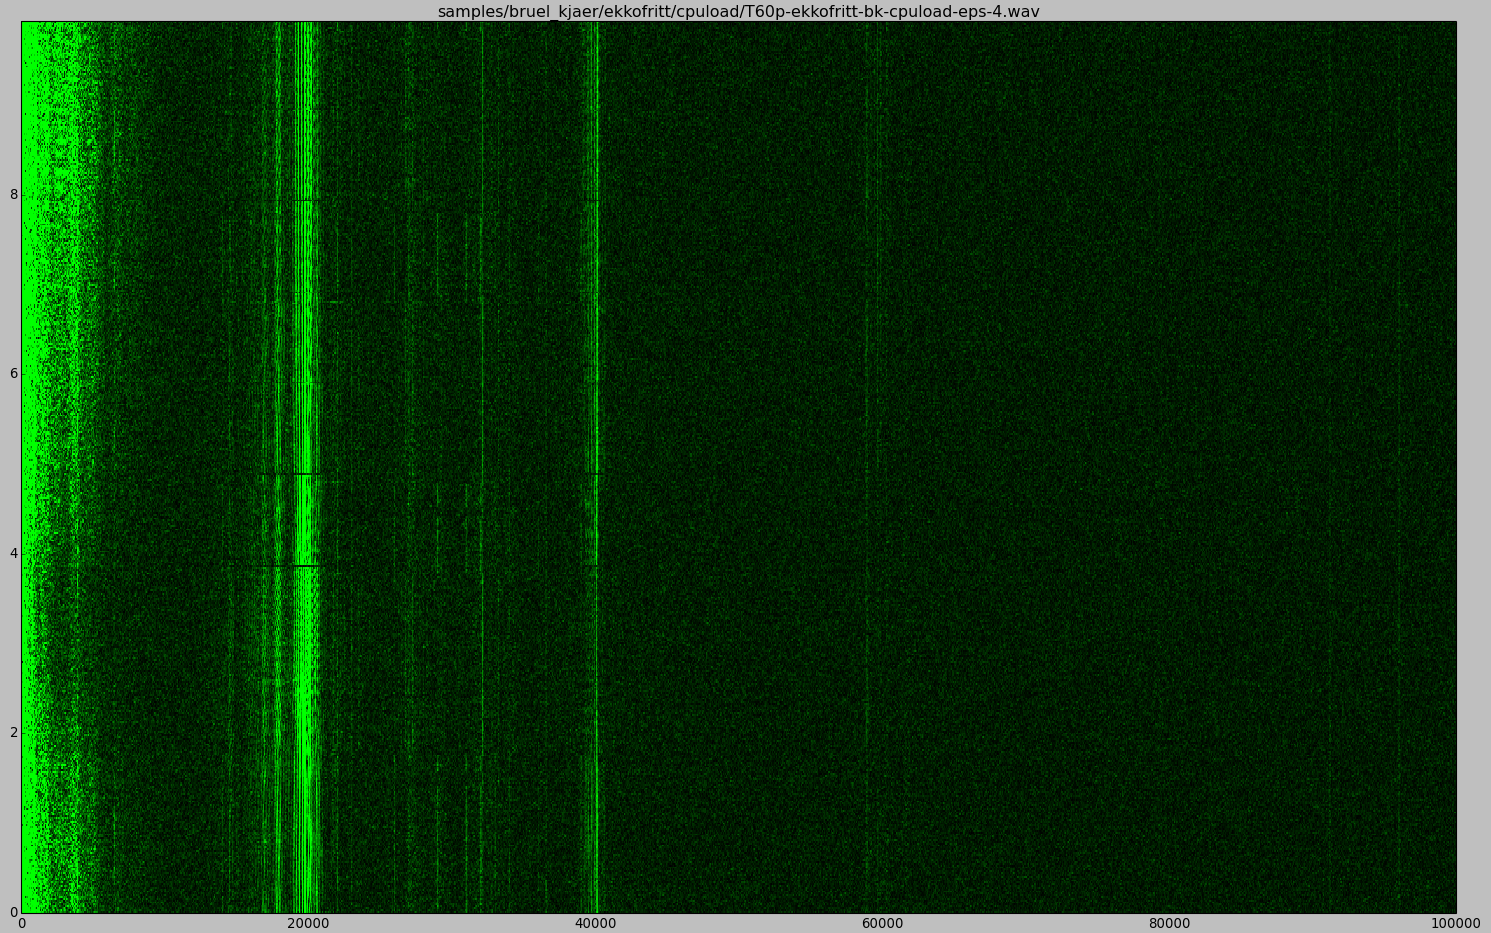
\includegraphics[width=1\linewidth]{T60p-ekkofritt-bk-cpuload-eps-4.png}
	    \caption{External power supply}
	    \label{fig:T60p-ekkofritt-bk-cpuload-eps-4}
    \end{subfigure}
    \begin{subfigure}{0.5\textwidth}
	    \centering
	    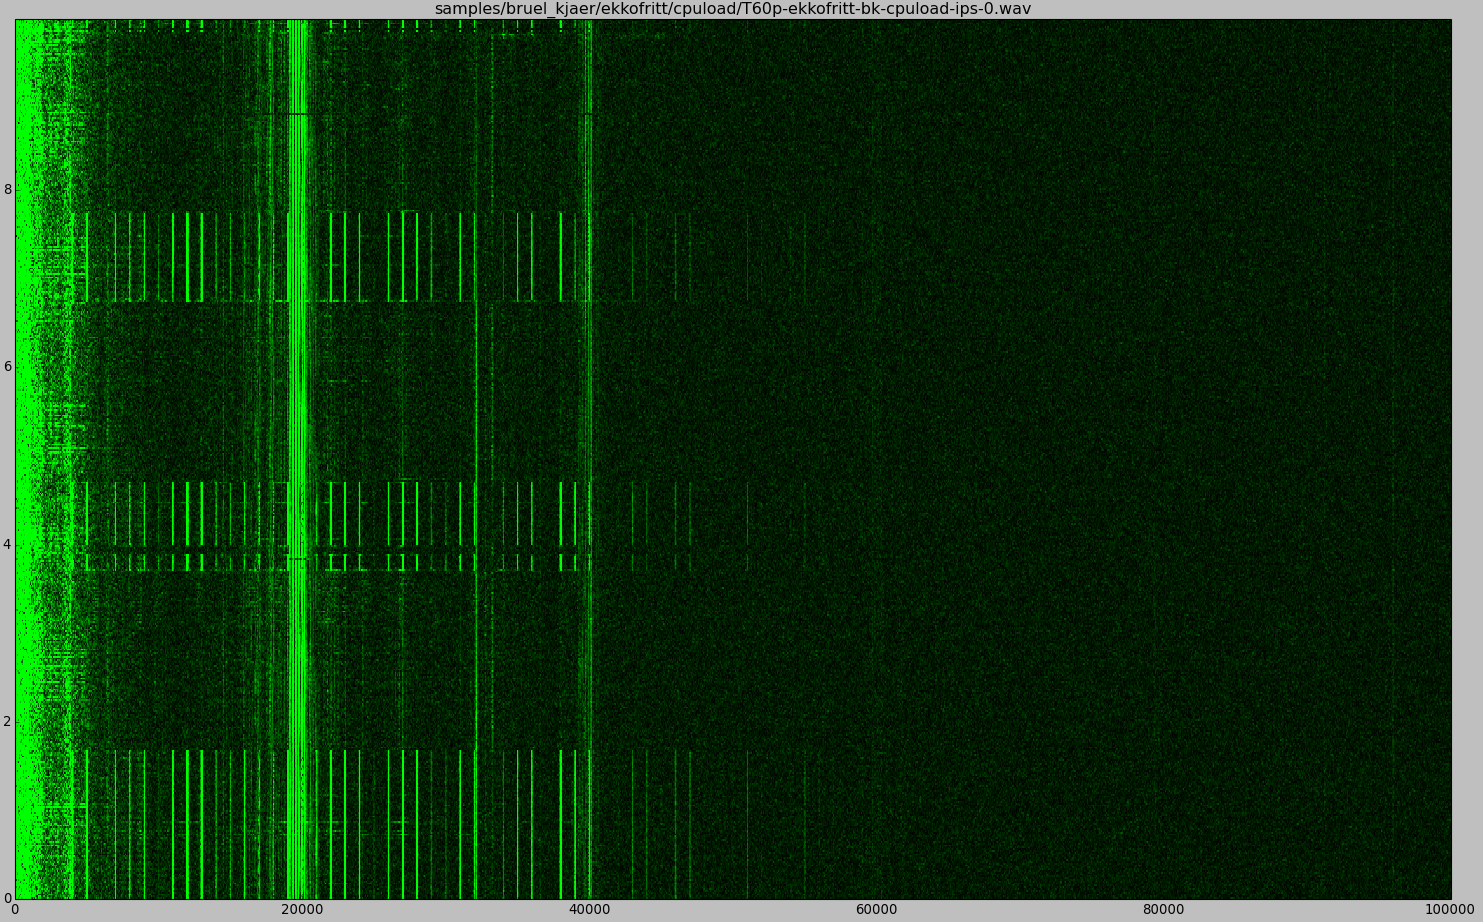
\includegraphics[width=1\linewidth]{T60p-ekkofritt-bk-cpuload-ips-0.png}
	    \caption{Internal power supply}
	    \label{fig:T60p-ekkofritt-bk-cpuload-ips-0}
    \end{subfigure}
    \caption{Acoustic recording (10 sec, 0-100kHz) of the Lenovo T60p when running a full CPU load. The recording was made in an anechoic chamber using the Brüel\&Kjær 4939 microphone with the NI myDAQ.}
	\label{fig:T60p-ekkofritt-bk-cpuload}
\end{wrapfigure}


\begin{wrapfigure}{r}{1\textwidth}
    \centering
    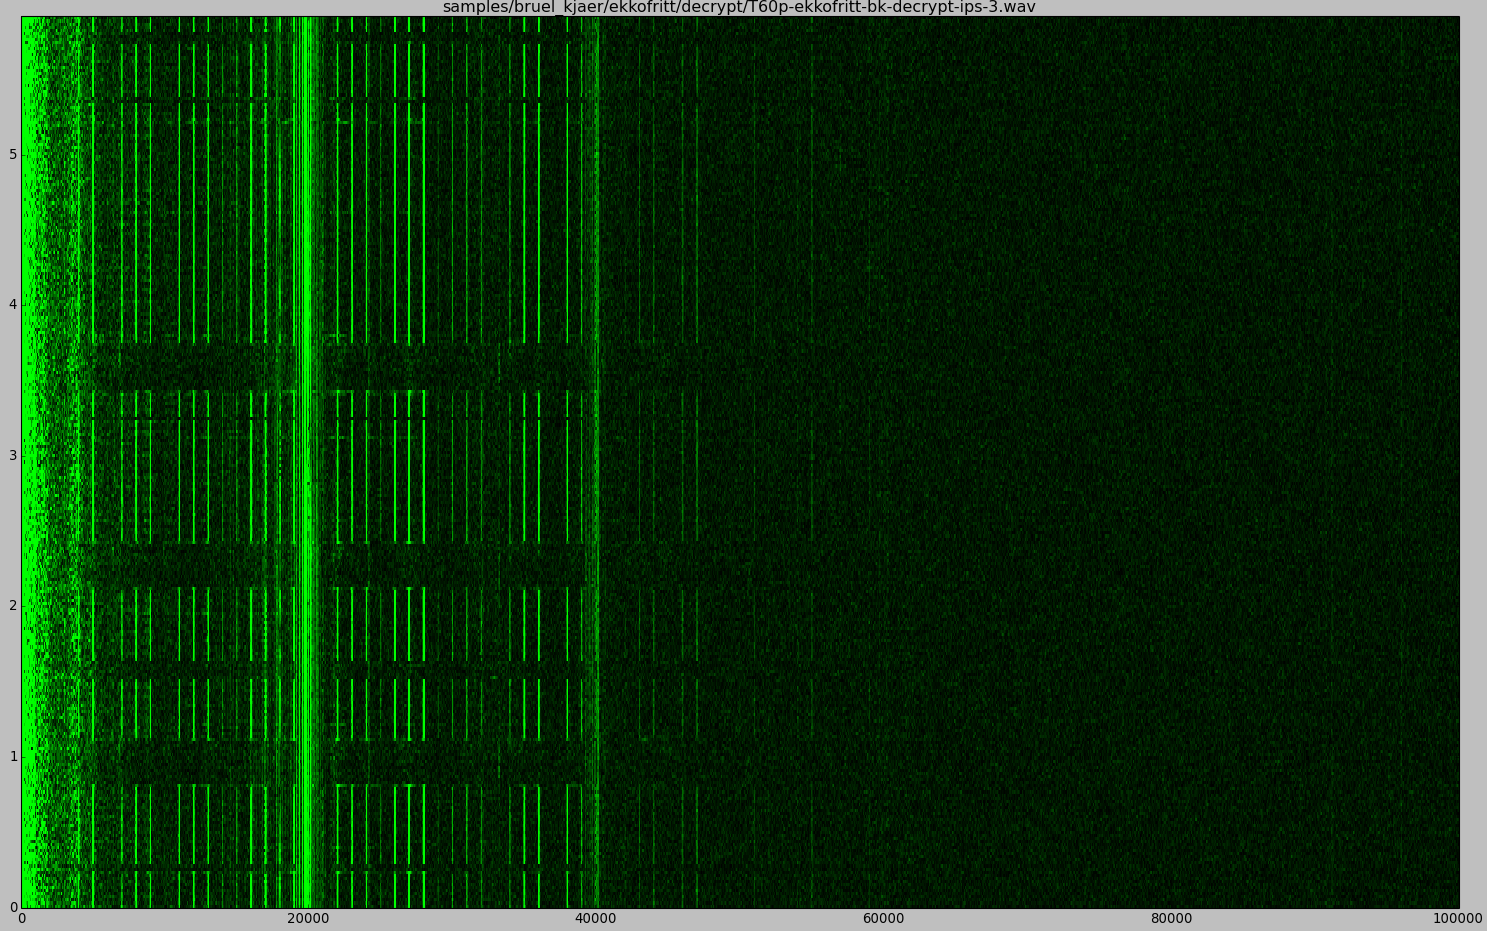
\includegraphics[width=1\linewidth]{T60p-ekkofritt-bk-decrypt-ips-3.png}
    \caption{Acoustic recording (6 sec, 0-100kHz) of the Lenovo T60p when running a dycrypt. The recording was made in an anechoic chamber using the Brüel\&Kjær 4939 microphone with the NI myDAQ. }
    \label{fig:T60p-ekkofritt-bk-decrypt-ips-3}
\end{wrapfigure}

\begin{wrapfigure}{r}{1\textwidth}
    \centering
    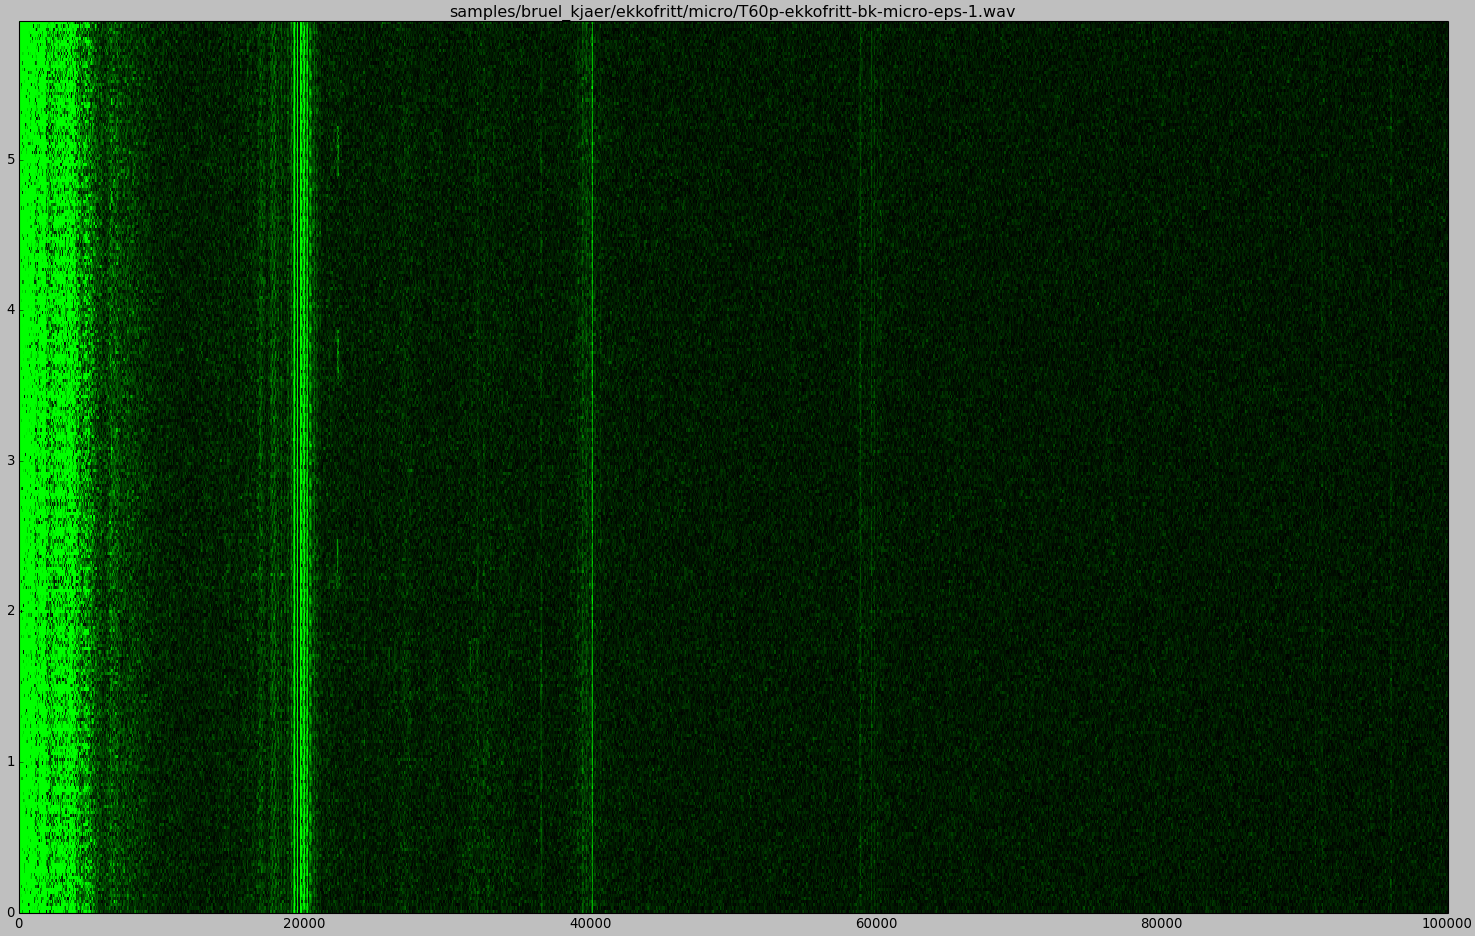
\includegraphics[width=1\linewidth]{T60p-ekkofritt-bk-micro-eps-1.png}
    \caption{Acoustic recording (6 sec, 0-100kHz) of the Lenovo T60p when running micro. The recording was made in an anechoic chamber using the Brüel\&Kjær 4939 microphone with the NI myDAQ. }
    \label{fig:T60p-ekkofritt-bk-micro-eps-1}
\end{wrapfigure}

\begin{wrapfigure}{r}{1\textwidth}
    \centering
    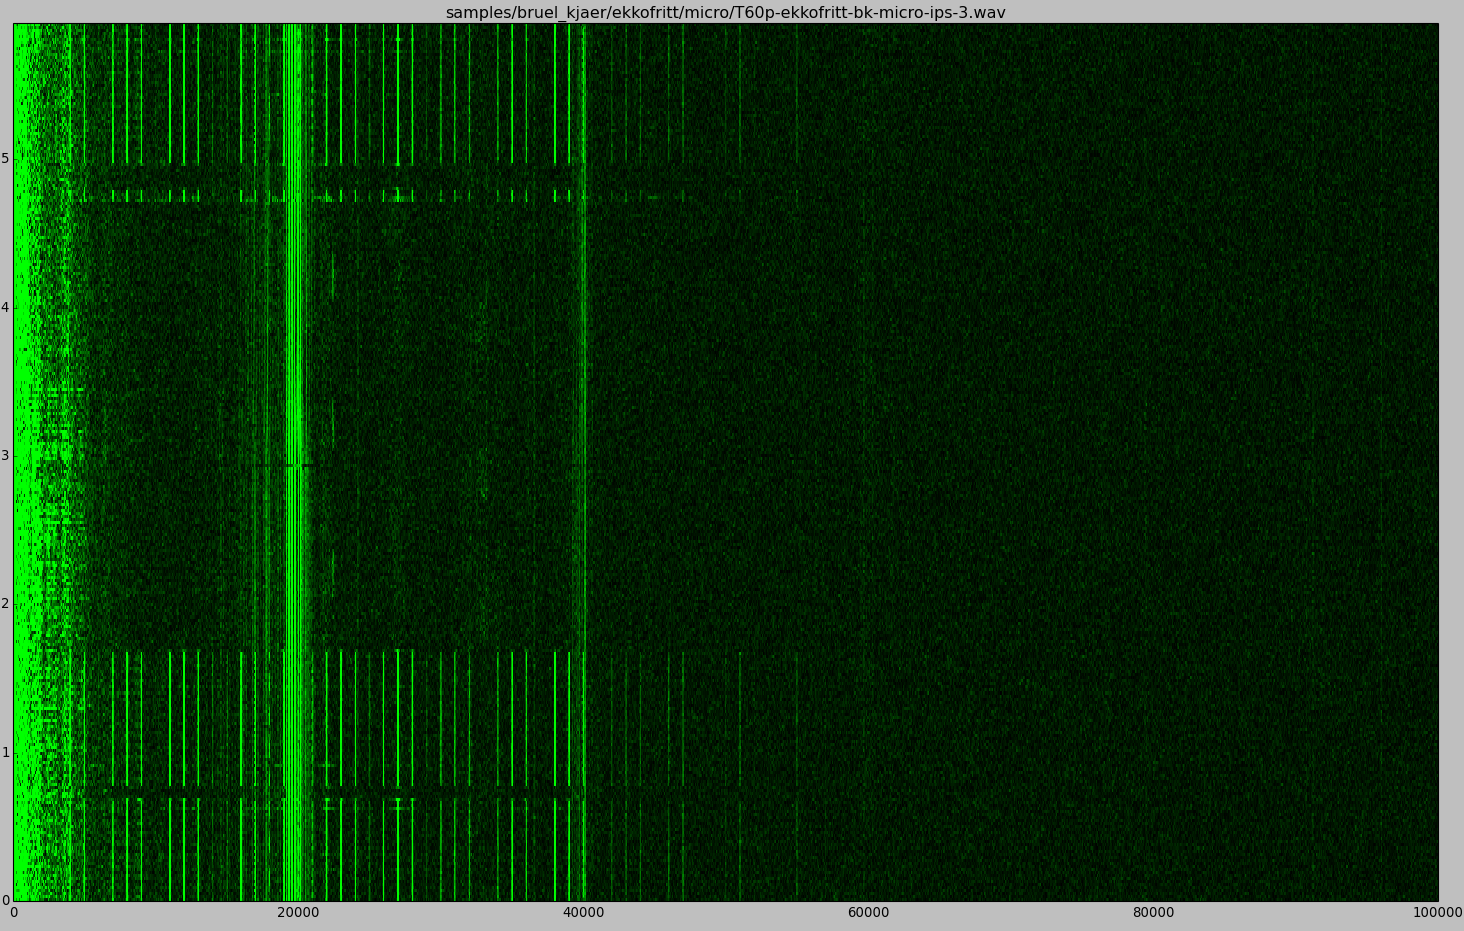
\includegraphics[width=1\linewidth]{T60p-ekkofritt-bk-micro-ips-3.png}
    \caption{Acoustic recording (6 sec, 0-100kHz) of the Lenovo T60p when running micro. The recording was made in an anechoic chamber using the Brüel\&Kjær 4939 microphone with the NI myDAQ. }
    \label{fig:T60p-ekkofritt-bk-micro-ips-3}
\end{wrapfigure}

\begin{wrapfigure}{r}{1\textwidth}
    \centering
    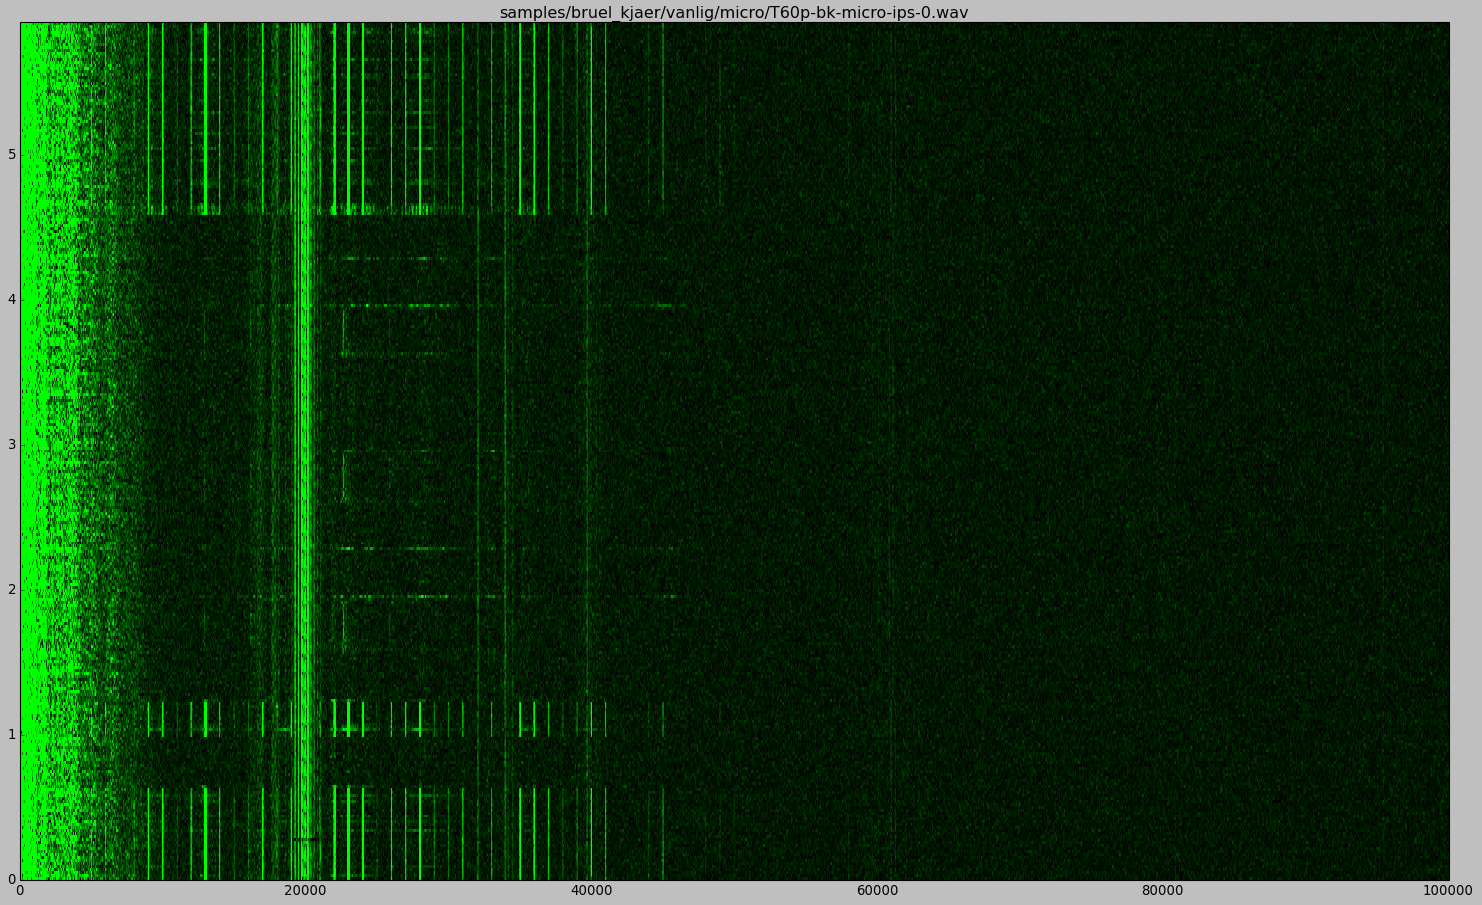
\includegraphics[width=1\linewidth]{T60p-bk-micro-ips-0.png}
    \caption{Acoustic recording (6 sec, 0-100kHz) of the Lenovo T60p when running micro. The recording was made using the Brüel\&Kjær 4939 microphone with the NI myDAQ. }
    \label{fig:T60p-bk-micro-ips-0}
\end{wrapfigure}

\begin{wrapfigure}{r}{1\textwidth}
	\begin{subfigure}{0.5\textwidth}
	    \centering
	    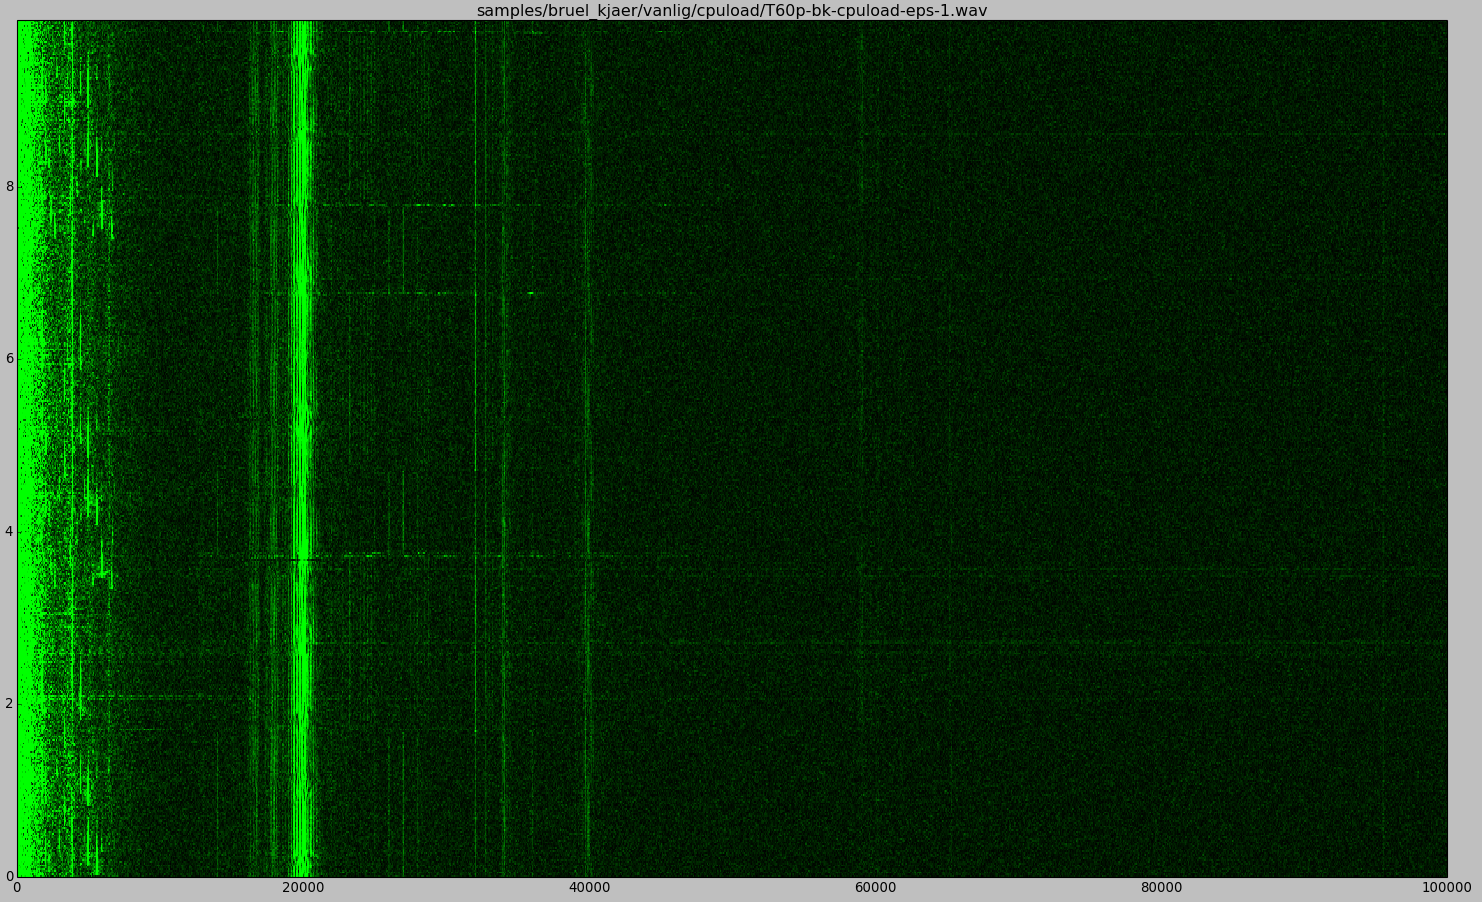
\includegraphics[width=1\linewidth]{T60p-bk-cpuload-eps-1.png}
	    \caption{External power suply}
	    \label{fig:T60p-bk-cpuload-eps-1-1a}
    \end{subfigure}
    \begin{subfigure}{0.5\textwidth}
	    \centering
	    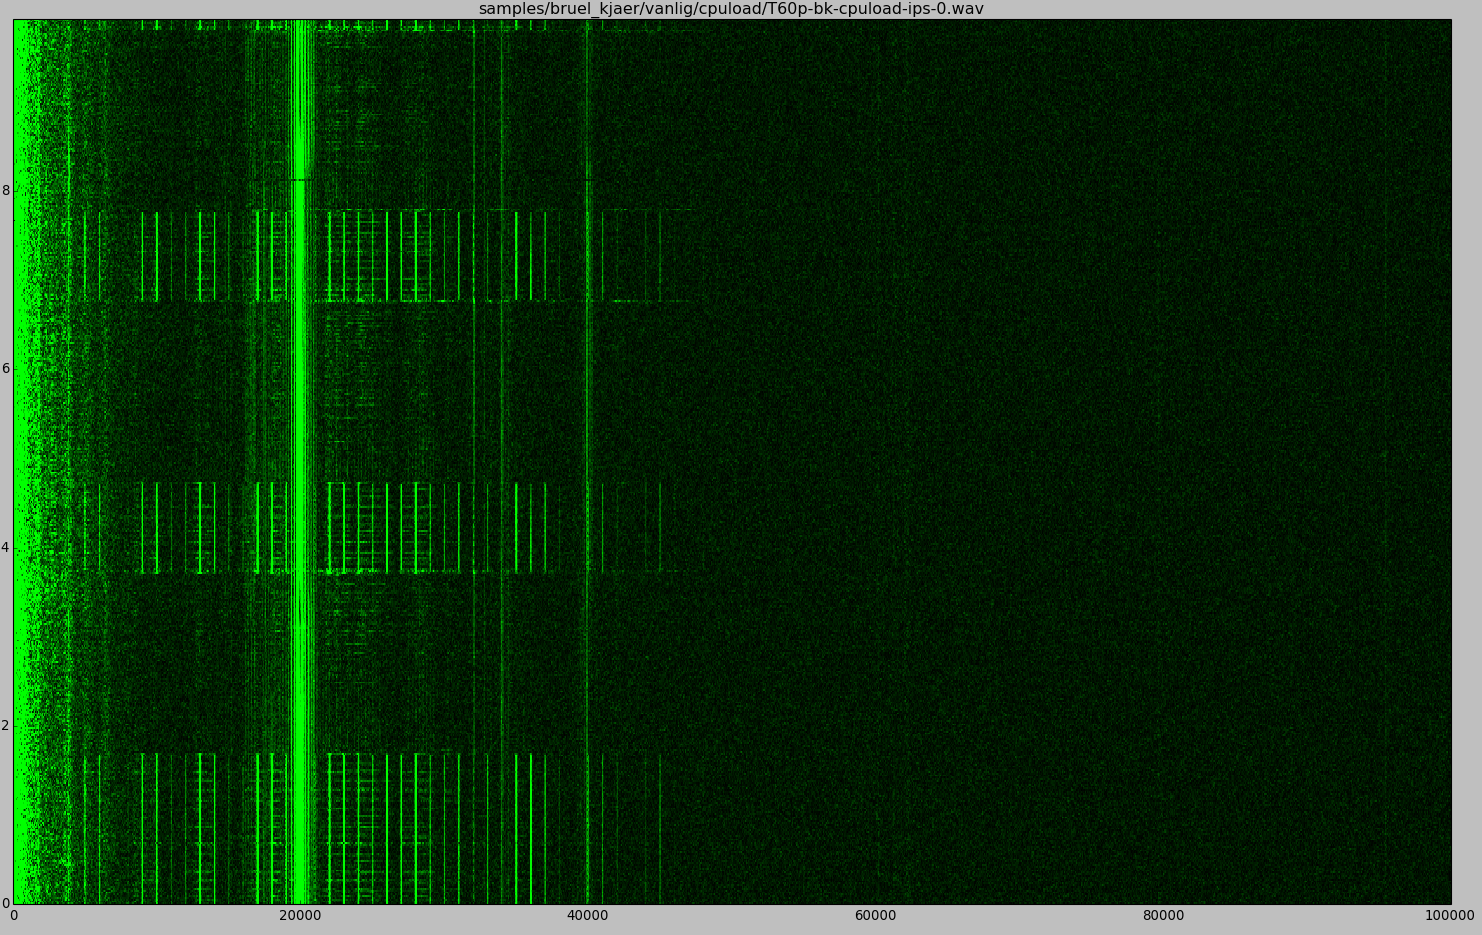
\includegraphics[width=1\linewidth]{T60p-bk-cpuload-ips-0.png}
	    \caption{Internal power suply}
	    \label{fig:T60p-bk-cpuload-ips-0-1b}
    \end{subfigure}
    \caption{Acoustic recording (10 sec, 0-100kHz) of the Lenovo T60p when running a full CPU load. The recordings was made using the Brüel\&Kjær 4939 microphone with the NI myDAQ. }
	\label{fig:T60p-bk-cpuload}
\end{wrapfigure}

